\section{Correction method}
\label{sec:correction_method}
With the knowledge of what might be the source of the artifacts seen in the temperature recording, it is chosen to find a way to compensate and correct the recording.
Jumps occur in each region of interest at the same time and are shown by a high difference of the values between two frames. The amount of the observed jumps varies between 0 and 20 in the recordings. Furthermore the appearance of the jumps is non-periodic and in each recording at different time points and interval.
\begin{figure}[H]
	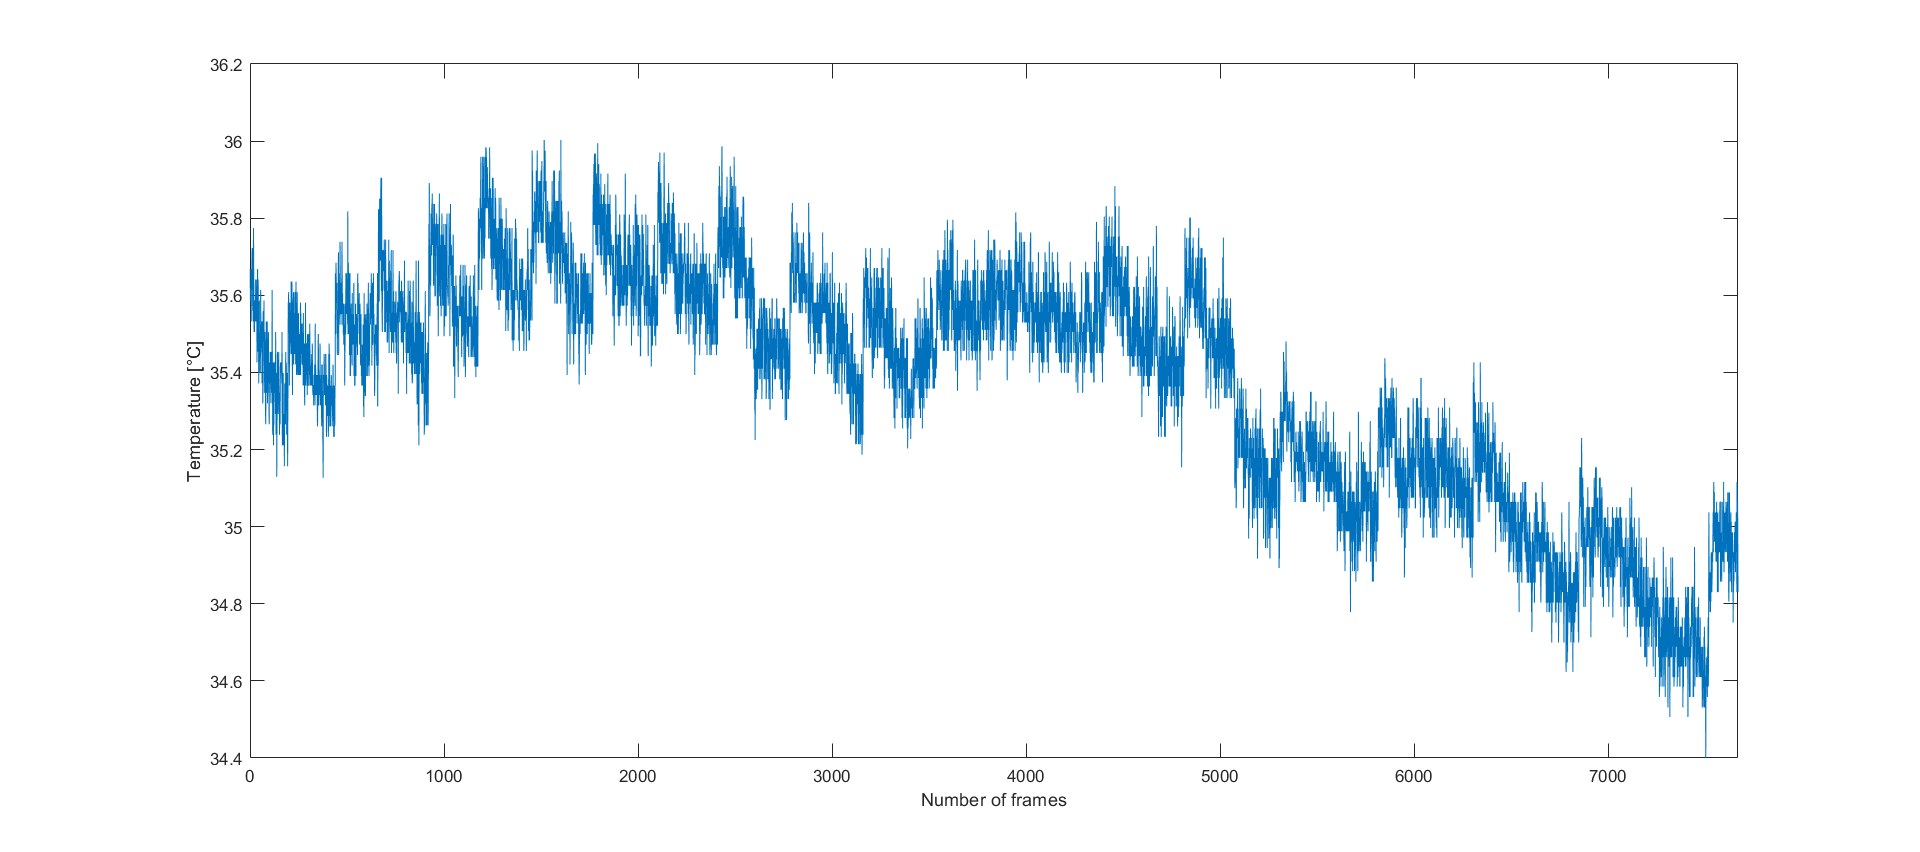
\includegraphics[width=1\textwidth]{figures/raw15}
	\caption{The original data of region 15 in the uncuffed recording of subject 1 including 20 jumps.}
	\label{fig:raw15}
\end{figure}
%A continuous wavelet transform show the time frequency analysis content of the data for each region. Frequencies of higher magnitude will show up with brighter colors, which can also be seen on the magnitude colorbar for comparison of the magnitude in values. 
%The freqency of the scalograms vary from 2.7370 Hz to 0.0031 Hz. This means according to the litterature that bands of cardiac, repiratory, endothelial, myogenic and neurogenic is represented in the wavelet frequency span for the time frequency analysis. \cite{sagaidachnyi2014}
%\begin{figure}[H]
%	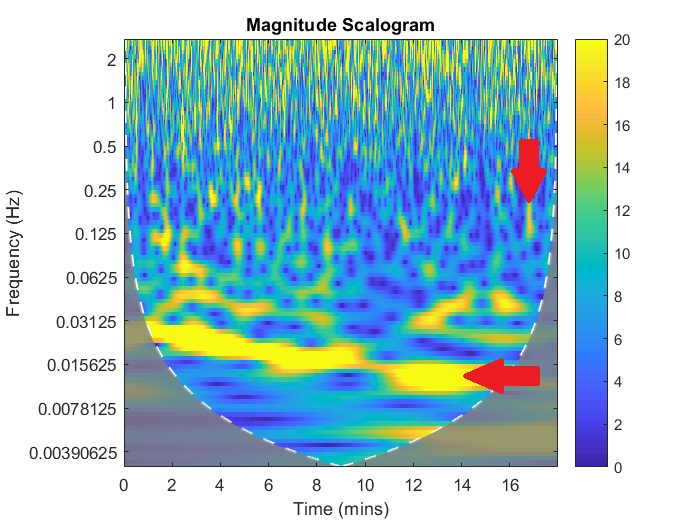
\includegraphics[width=0.7\textwidth]{figures/scalogram_uncorr}
%	\caption{Scalogram from the original data of region 15 in the uncuffed recording of subject 1, where high spike magnitudes can be seen induced by the jumps.}
%	\label{fig:scalogram_uncorr}
%\end{figure}
From the raw data magnitude of the scalogram show high magnitude peaks exactly at the same time points where the jumps are occurring, which can be seen in figure \ref{fig:scalogram_uncorr}. Due to this falsifying of the magnitude, the results of the data analysis are also falsified.\fxnote{We cannot ref to a figure that comes 4 pages later...}

Additionally there is also a drift occurring within each interval between two jumps, which hampers the correct data analysis, this can also be seen in figure \ref{fig:scalogram_uncorr} as the frequency band with higher magnitude. To reduce the drift component and the jumps in the signals, the two following correction methods have been compiled, whereby the second one has been implemented.

\textbf{Method 1: Regression of first interval}

The first implemented method is based on the assumption that the drift is equal in each interval. It is also assumed that the thermal camera has been calibrated just before the recording, so the first interval can be used as a reference to calculate the drift component. Therefore a linear regression for the first interval has been made. With the resultant slope $m$ follows the calculation of the drift difference $d$ within the first interval. Due to the assumption, that the drift difference is equal, the slope of the drift of each interval depends on the length of the interval. The slopes have been calculated with equation \ref{eq:slope}.
\begin{flalign}
	m=\frac{d}{length(interval)}
	\label{eq:slope}
\end{flalign}
To compensate for the drift, a straight with the inverse slope and starting point in the first data point of the interval has been calculated. The middle points between the original data and the new calculated straight build the correction of the data signal.
\begin{figure}[H]
	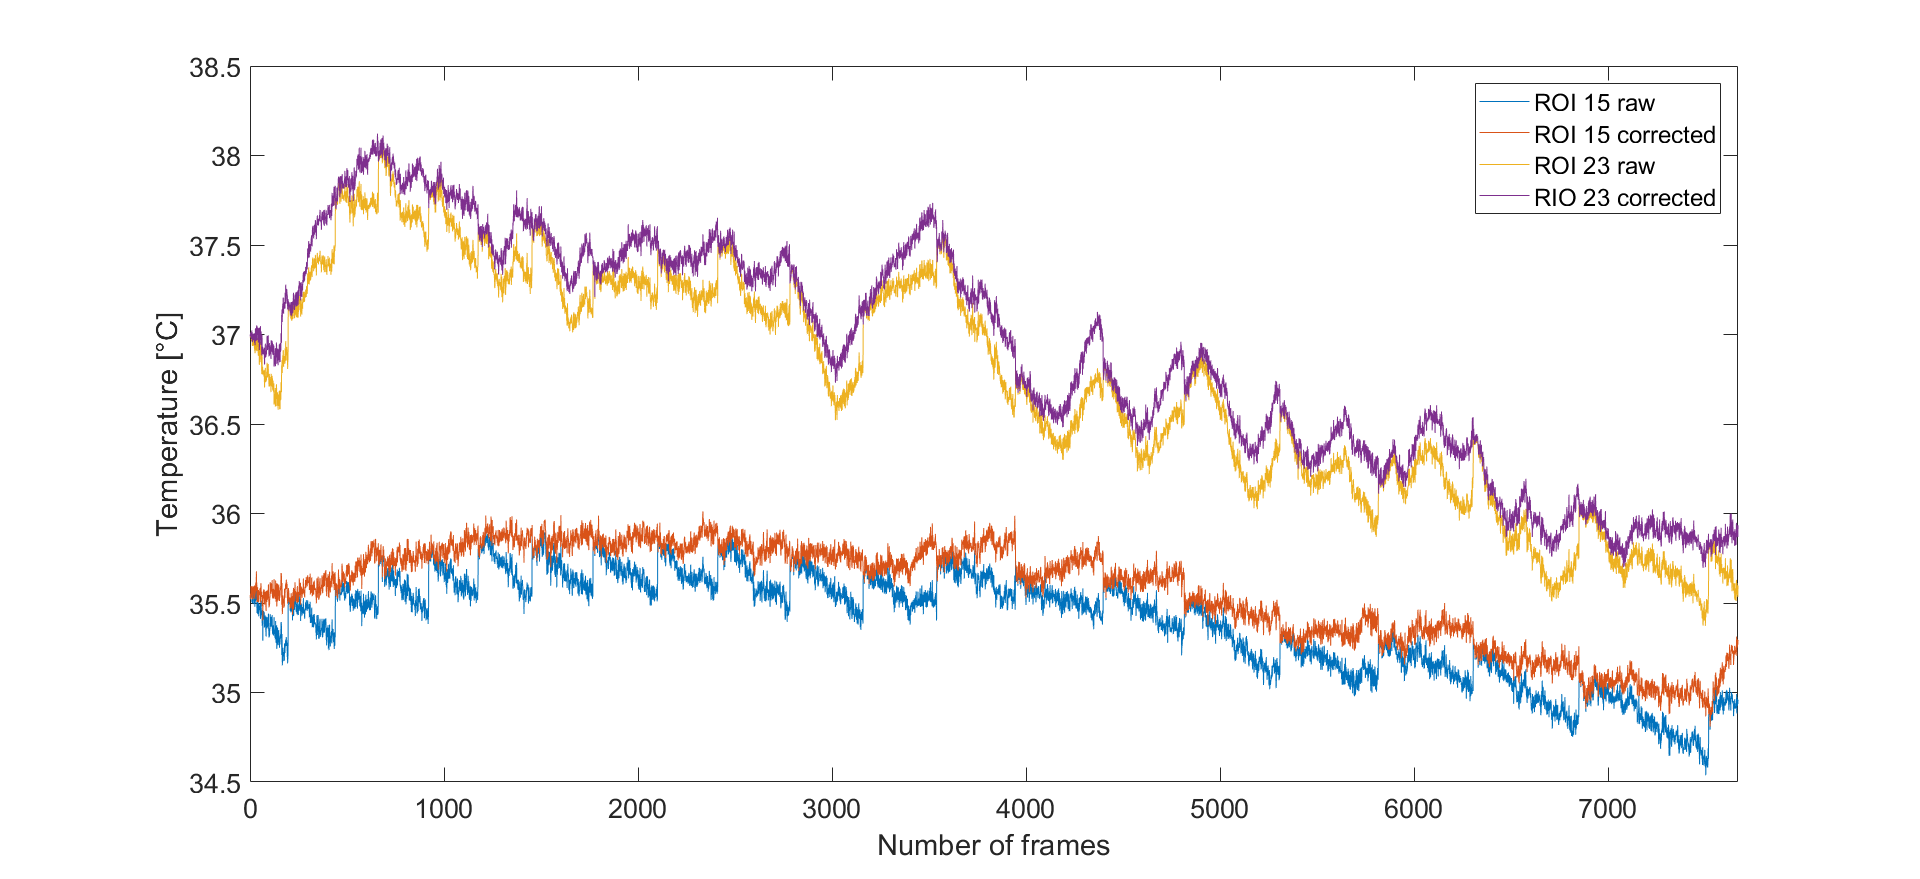
\includegraphics[width=1\textwidth]{figures/old_correction_sub1}
	\caption{The original data of ROI 15 in blue and ROI 23 in yellow. Applied correction of ROI 15's data in red and ROI 23's data in purple.}
	\label{fig:oldcorr}
\end{figure}
As it can be seen in figure \ref{fig:oldcorr} this correction only worked partially where several parts showed less drift and lower jumps. Through the method worked at some parts it still had a lot of weak points. Primarily because some jumps had been strengthened. Due to the outcome of this method, the assumption, that the drift is equal in each interval has been discarded. 

\textbf{Method 2: Regression of each interval}

The second implemented method is due to the failure of the first method based on the assumption that the drift is not equal in each interval. Out of the recorded data the exact drift is indeterminable. Hence a method which tries to fit the separate intervals together without the necessity of the awareness of the real drift component and avoids the suppression of the basic shape of the signal has been chosen.
Therefore firstly the linear regressions for all intervals and the corresponding residuals are calculated.
The idea is to move the end point of a regression line and the start point of the next regression line together. Thus the middle points between end and following start point are calculated. The alignment of the regression lines is changed, so that the start and end points of all the new created orientation straights fit the middle points, except the first and the last orientation straight. Both fit just one middle point. The start of the first orientation straight is the start point of the regression line of the first interval and the end point of the last orientation straight is the end point of the regression line of the last interval.
\begin{figure}[H]
	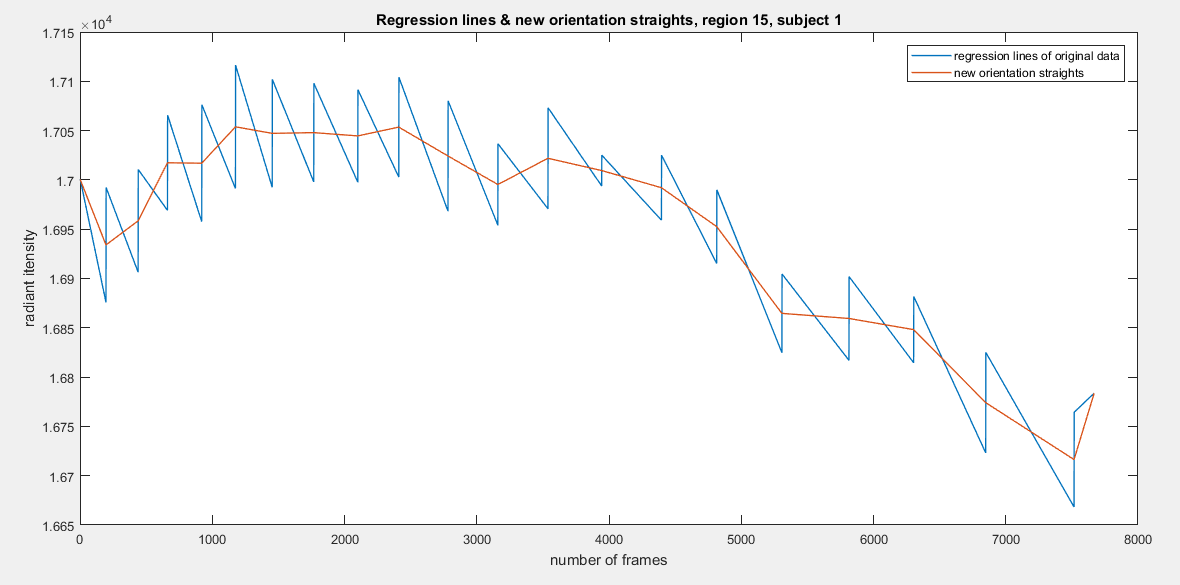
\includegraphics[width=0.9\textwidth]{figures/reg15}
	\caption{Connected regression lines of the original data of region 15 in the uncuffed recording of subject 1 in blue. New created orientation line of the same recording in the same region shown in red.}
	\label{fig:reg15}
\end{figure}
As shown in figure \ref{fig:reg15} the new orientation straight fits the regression lines together without suppressing the shape of the signal. Subsequently the residuals have been added to the new orientation straight, to sustain the ratio between the data points. Figure \ref{fig:corr15} shows the corrected signal wherein the jumps, separated intervals, have been connected and the jumps have been largely corrected.
\begin{figure}[H]
	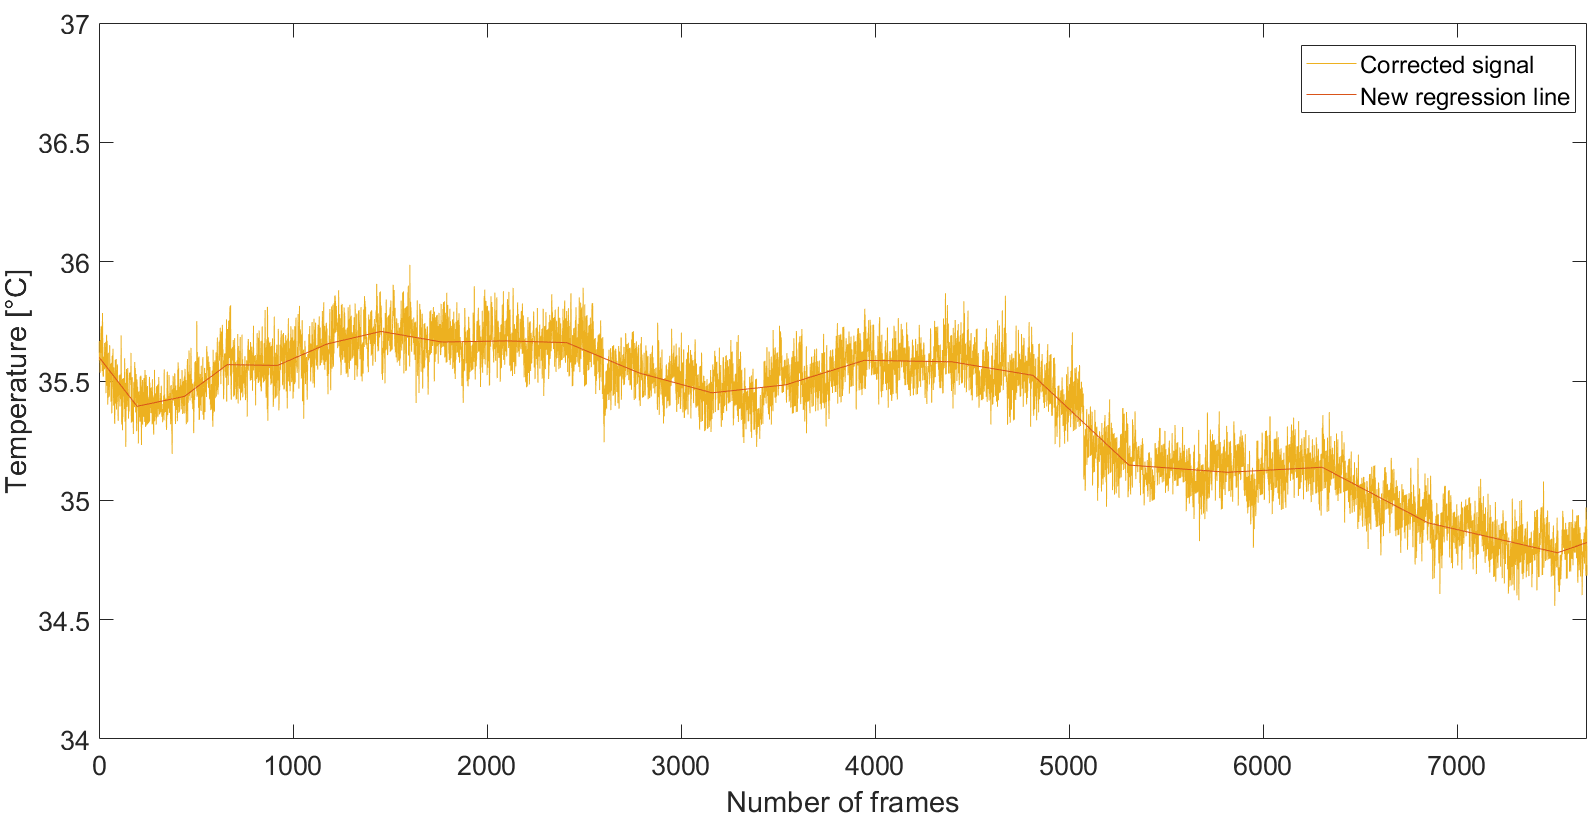
\includegraphics[width=0.9\textwidth]{figures/corr15}
	\caption{Orientation line based on the data of the uncuffed recording of subject 1 in region 15 shown in red. Corrected signal of the same data in yellow.}
	\label{fig:corr15}
\end{figure}
%After the drift correction is added to the signal, the energy has been reduced at these areas induced from the jump which can be seen in figure \ref{fig:scalogram_corr}. 
%\begin{figure}[H]
%	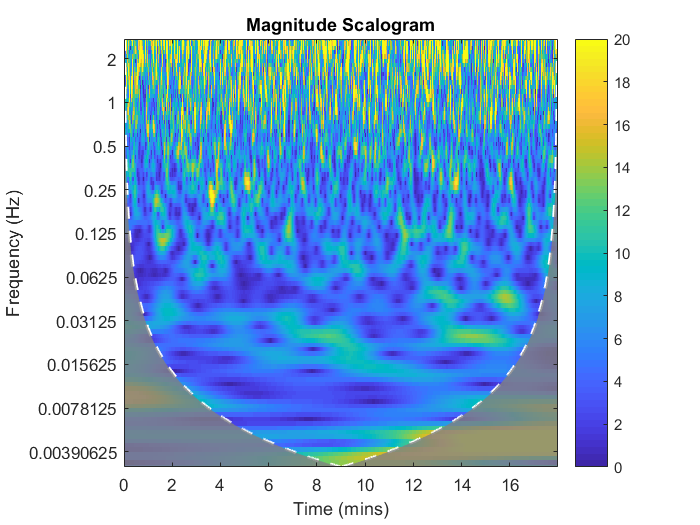
\includegraphics[width=1\textwidth]{figures/scalogram_corr}
%	\caption{Scalogram from the corrected data of region 24 in the cuffed recording of subject 1, where a dampening of the high spike and drift magnitudes induced by the jumps has been achieved.}
%	\label{fig:scalogram_corr}
%\end{figure} 
However, this method still has weak points. In figures \ref{fig:raw15} - \ref{fig:corr15} region of interest is located in the center of the thermal image. Regions which are located in the outer area of the thermal image show a few jumps after the correction which are bigger than before, illustrated on \figref{fig:corr23}. These extended jumps are due to the fact that the thermal image is more unstable in the outer areas than in the center, thus the pixel drift is increasing with increasing distance to the center of the thermal image. That means that in the corrected data of ROIs located in the outer areas of the thermal image still artifacts occur. 
\begin{figure}[H]
	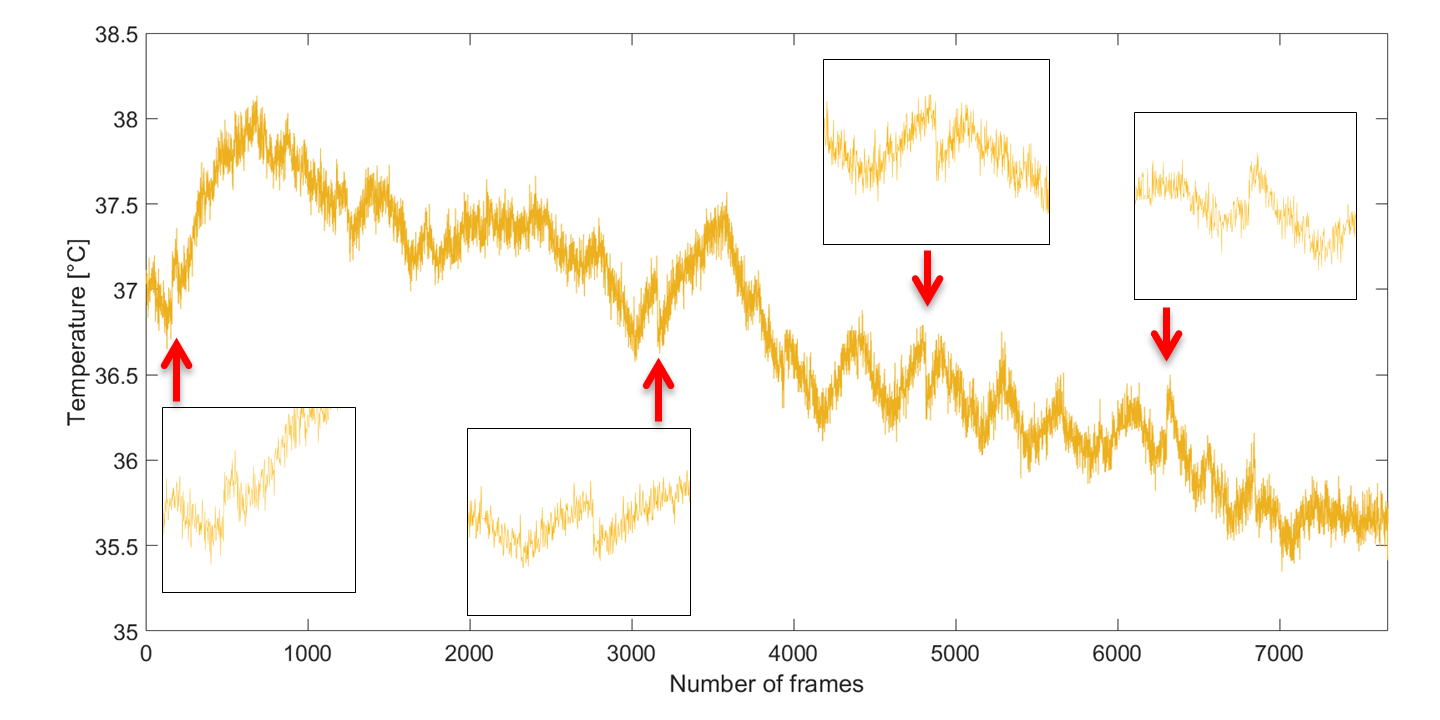
\includegraphics[width=0.9\textwidth]{figures/corr23pfeile}
	\caption{Corrected data of the uncuffed recording of subject 1 in region 23 shown in yellow. Red arrows show the jumps in this signal.}
	\label{fig:corr23}
\end{figure}